%
% mathematical_model.tex
%

\section{Математическая модель}


\subsection{Функционал свободной энергии}
%----------------------------------------------------

Для начала определим функционал свободной энергии, $\Psi$, который является функцией от фазового поля $\phi$ и её производных:

\begin{equation} \label{energ}
\Psi[\phi] = \int\limits_V \left( \frac{\alpha}{2}\phi^2 + \frac{\beta}{2}(\nabla \phi)^2 + \frac{\gamma}{2}(\Delta \phi)^2 + U(\phi) \right) dV,
\end{equation}
где~$\alpha$, $\beta$ и $\gamma$~--- коэффициенты, характеризующие энергию взаимодействия между частицами и влияние пространственных изменений фазовой функции; $U(\phi)$~--- потенциал, зависящий только от фазового поля $\phi$. \\
Вид выражения~($\ref{energ}$) для свободной энергии может быть обоснован теоретически~\cite{chen_2002} и зависит от вида потенциала взаимодействия между атомами решетки. 

\subsection{Вариация функционала свободной энергии}

Равновесное состояние системы в области $V$ соответствует минимуму функционала свободной энергии. Необходимым условием минимума является равенство нулю первой вариации $\delta \Psi$ функционала $\Psi$.

Для её вычисления рассмотрим изменение функционала свободной энергии при небольшом изменении $\phi \rightarrow \phi + \delta \phi$:
\begin{equation*}
    \delta \Psi = \Psi[\phi + \delta \phi] - \Psi[\phi].
\end{equation*}


После подстановки и разложения до первого порядка по $\delta \phi$, получаем:
\begin{equation*}
    \delta \Psi = \int \limits_V \left( \alpha \phi \delta \phi + \beta \nabla \phi \cdot \nabla (\delta \phi) + \gamma \Delta \phi \Delta (\delta \phi) +  \frac{dU}{d\phi} \delta \phi \right) dV.
\end{equation*}

Для членов, содержащих градиенты и лапласианы, применяем интегрирование по частям. Будем считать, что на границе $\partial V$ области $V$ заданы граничные условия
\begin{equation} \label{gran}
    \delta \phi \bigg|_{\partial V} = ( \Vec{n} \cdot \nabla (\delta \phi)) \bigg|_{\partial V}= 0,
\end{equation}
где $\Vec{n}$~--- единичная нормаль к границе $\partial V$ области $V$. В этом случае граничные слагаемые обращаются в ноль.
Для градиентного члена имеем:
\begin{equation*}
\int \limits_V \beta \nabla \phi \cdot \nabla (\delta \phi) \, d V.
\end{equation*}
Применим интегрирование по частям, используя теорему Остроградского-Гаусса:
\begin{align*}
\int \limits_V \beta \nabla \phi \cdot \nabla (\delta \phi) \, d V = -\int \limits_V \beta \delta \phi \, \Delta \phi \, d V + \underbrace{\oint \limits_{\partial V} \beta \delta \phi \, (\nabla \phi \cdot d\mathbf{S})}_{=0} 
= -\int \limits_V \beta \delta \phi \, \Delta \phi \, d V.
\end{align*}

Теперь рассмотрим выражение с лапласианами:
\begin{equation*}
\int \limits_V \gamma \Delta \phi \Delta (\delta \phi) \, d V.
\end{equation*}
Для него применим интегрирование по частям дважды:

\begin{multline*}
\int \limits_{V} \gamma \Delta \phi \Delta (\delta \phi) \, d V = \int \limits_{V} \gamma \nabla \cdot (\nabla \phi) \nabla \cdot (\nabla (\delta \phi)) \, d V =\\
= -\int \limits_{V} \gamma \nabla (\nabla \cdot (\nabla \phi)) \cdot \nabla (\delta \phi) \, d V + \oint \limits_{\partial V} \gamma (\nabla \cdot (\nabla \phi)) (\nabla (\delta \phi) \cdot d\mathbf{S}) =\\
= \int \limits_{V} \gamma \Delta^2 \phi \delta \phi \, d V - 
\underbrace{\oint \limits_{\partial V} \gamma \nabla (\Delta \phi) \cdot (\delta \phi d\mathbf{S})}_{=0} + \underbrace{\oint \limits_{\partial V} \gamma (\Delta \phi) (\nabla (\delta \phi) \cdot d\mathbf{S})}_{=0} = \int \limits_{V} \gamma \Delta^2 \phi \delta \phi \, d V.
\end{multline*}
    
Теперь, подставляя результаты интегрирования по частям и учитывая вариацию потенциала $U(\phi)$, приходим к выражению:

\begin{equation} \label{delta psi}
    \delta \Psi = \int \limits_V \left( \alpha \phi - \beta \Delta \phi + \gamma \Delta^2 \phi + \frac{dU}{d\phi} \right) \delta \phi \, dV.
\end{equation}
Таким образом, стационарное распределение фазового поля должно удовлетворять уравнению Эйлера-Лагранжа:
\begin{equation*}
    \phi = \operatorname{argmin} \Psi(\phi) \Leftrightarrow \delta \Psi[\phi, \delta \phi] = 0,
\end{equation*}
для любых достаточно гладких $\delta \phi$, удовлетворяющих граничным условиям~($\ref{gran}$).

В силу произвольности $\delta \phi$ отсюда следует, что  $\phi$ удовлетворяет уравнению 
\begin{equation} \label{ravnov_eq}
    \alpha \phi - \beta \Delta \phi + \gamma \Delta^2 \phi + \frac{dU}{d\phi} = 0.
\end{equation}
Решение этого уравнения совместно с заданными граничными условиями нужного вида определяет стационарное распределение $\phi$.


\subsection{Уравнение эволюции}
%----------------------------------------------------
%Уравнение Эволюции---------------------------------------------------
Динамику фазового поля $\phi$ по времени описывает уравнение эволюции~\cite{chen_2002, elder_2002, elder_2004}
\begin{equation} \label{evolut_eq}
\frac{\partial \phi}{\partial t} = -\operatorname{div}\left[ -K \operatorname{grad}\left(\frac{\delta \psi}{\delta \phi}\right)\right],
\end{equation}
где $K > 0$~--- феноменологическая константа; $\delta \psi / \delta \phi$~--- функциональная производная от свободной энергии.

Функциональная производная \( \delta \psi / \delta \phi \) и вариация \(\delta \Psi\)
связаны соотношением
\[
\delta \Psi = \int \limits_V \frac{\delta \psi}{\delta \phi} \delta \phi \, dV.
\]


Из уравнения~(\ref{delta psi}) следует что:
\[
\frac{\delta \psi}{\delta \phi} =  \alpha \phi - \beta \Delta \phi + \gamma \Delta^2 \phi + \frac{dU}{d\phi} .
\]

Подставляя функциональную производную в уравнение эволюции, мы получим:

\begin{equation*}
    \frac{\partial \phi}{\partial t} = \operatorname{div}\left[K \operatorname{grad}\left(\alpha \phi - \beta \Delta \phi + \gamma \Delta^2 \phi + \frac{dU}{d\phi}\right)\right].
\end{equation*}

Отсюда следует важный факт: фазовое поле $\phi$ является консервативной величиной. То есть: если система изолирована (нет потоков через границы) и отсутствуют внутренние источники или стоки, то интеграл $\phi$ по объему системы остается неизменным во времени.

Также можно показать, что при заданных граничных условиях~($\ref{gran}$), энергия системы убывает на решениях уравнения~(\ref{evolut_eq}), то есть 
\begin{equation*}
    \frac{d \Psi}{d t} \leqslant 0.
\end{equation*}

Уравнение~(\ref{evolut_eq}) имеет следующий смысл: при отклонении $\phi$ от равновесного решения, т. е. от решения уравнения~(\ref{ravnov_eq}), эволюция $\phi$ направлена на компенсацию этого отклонения.
При этом правая часть уравнения~($\ref{ravnov_eq}$) имеет смысл обобщенной термодинамической силы, она <<возвращает>> $\phi$ в состояние, соответствующее локальному минимуму энергии~($\ref{energ}$).

\subsection{Потенциал $U(\phi)$}

Потенциал $U(\phi)$ задаётся в виде функции, чей вид, совместно с дифференциальными членами в~($\ref{energ}$) и в~($\ref{delta psi}$) обеспечивает существование нетривиальных решений, отличных от постоянных.

Будем использовать двухъямный полиномиальный потенциал:

\begin{equation*}
U(\phi) = \frac{\epsilon}{4}(\phi^2 - 1)^2.
\end{equation*}

Тогда уравнение эволюции примет вид:

\begin{equation} \label{evolution_eq}
\frac{\partial \phi}{\partial t} = \operatorname{div}\left\{K \operatorname{grad}\left[ \alpha \phi - \beta \Delta \phi + \gamma \Delta^2 \phi  + \epsilon \phi (\phi^2 - 1)\right]\right\}.
\end{equation}

Это уравнение описывает динамику фазового поля $\phi$ во времени, учитывая взаимодействия между частицами, пространственные изменения фазы, а также потенциальный барьер между разными фазовыми состояниями.

Обратим внимание, что $U(\phi)$ имеет два минимума, соответствующие
значениям \mbox{$\phi=\pm1$}. Это~--- стандартная форма двухямного потенциала, обеспечивающего сосуществование двух чистых фаз, соответствующего состояниям $\phi=\pm1$ и гарантирующих их несмешение. Состояние однородной смеси (например, $\phi = 0$) является неустойчивым, см. рисунок~\ref{fig:potential}.

\begin{figure}[t!]
    \centering
    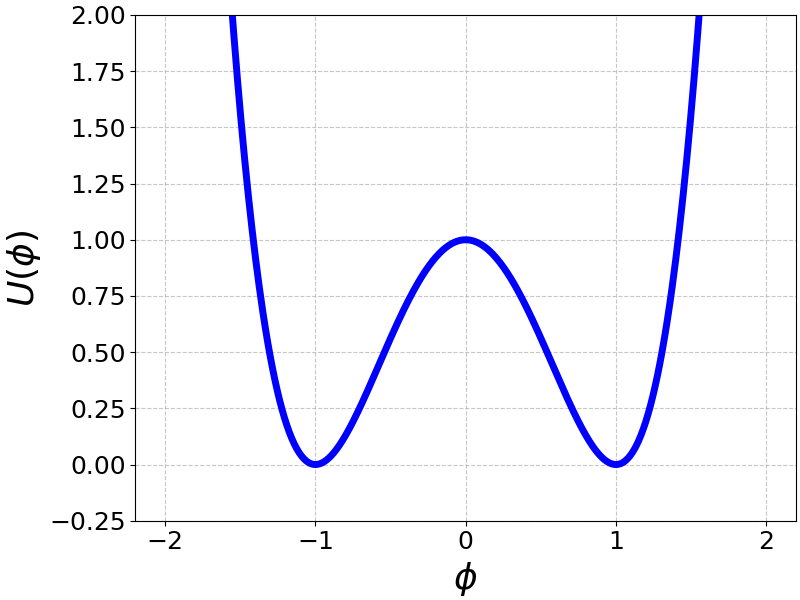
\includegraphics[width=0.6\linewidth]{images/potential.png}
    \caption{Вид потенциала при $\epsilon = 4$.}
    \label{fig:potential}
\end{figure}

